\section{Dielectric properties of metals}
\label{sec:Dielectric}

Many materials can be described using the Drude-Lorenz model. This model assumes that
the electrons behave as the classical harmonic oscillator

\begin{equation}
    \frac{d^2 x}{d t^2} + \frac{d}{m} \frac{dx}{dt} + \omega_{\mathrm{0}}^2x = -\frac{e}{m}E_{\mathrm{0}}\exp(-\mathrm{i}\omega t)
\end{equation}

but neglecting the potential term leading to the equation

\begin{equation}
    \frac{d^2 x}{d t^2} + \frac{d}{m} \frac{dx}{dt} + = -\frac{e}{m}E_{\mathrm{0}}\exp(-\mathrm{i}\omega t).
\end{equation}

From this idea of writing the motion of the electrons as free electrons, we can link the
current generated by the electric field to conductivity. In the context of optics, 
we convert this quantity to the dielectric function

\begin{gather}
    \epsilon_{r,D}' = 1 - \frac{\omega_{\mathrm{p}}^2}{\omega^2+\gamma_D^2} \\
    \epsilon_{r,D}'' =\frac{\omega_{\mathrm{p}}^2\gamma_D}{\omega^3+\omega\gamma_D^2}.
\end{gather}

When investigating the dielectric function of gold and silver (see \cref{fig:DielFuncAuS}), some differences from
the idealized model are observed. For instance, in the case of gold, the approximation of
electrons in the energy range above \SI{2}{\eV} is not valid. However, for silver in the optical
range, the approximations hold true.

\begin{figure}[ht]
    \centering
    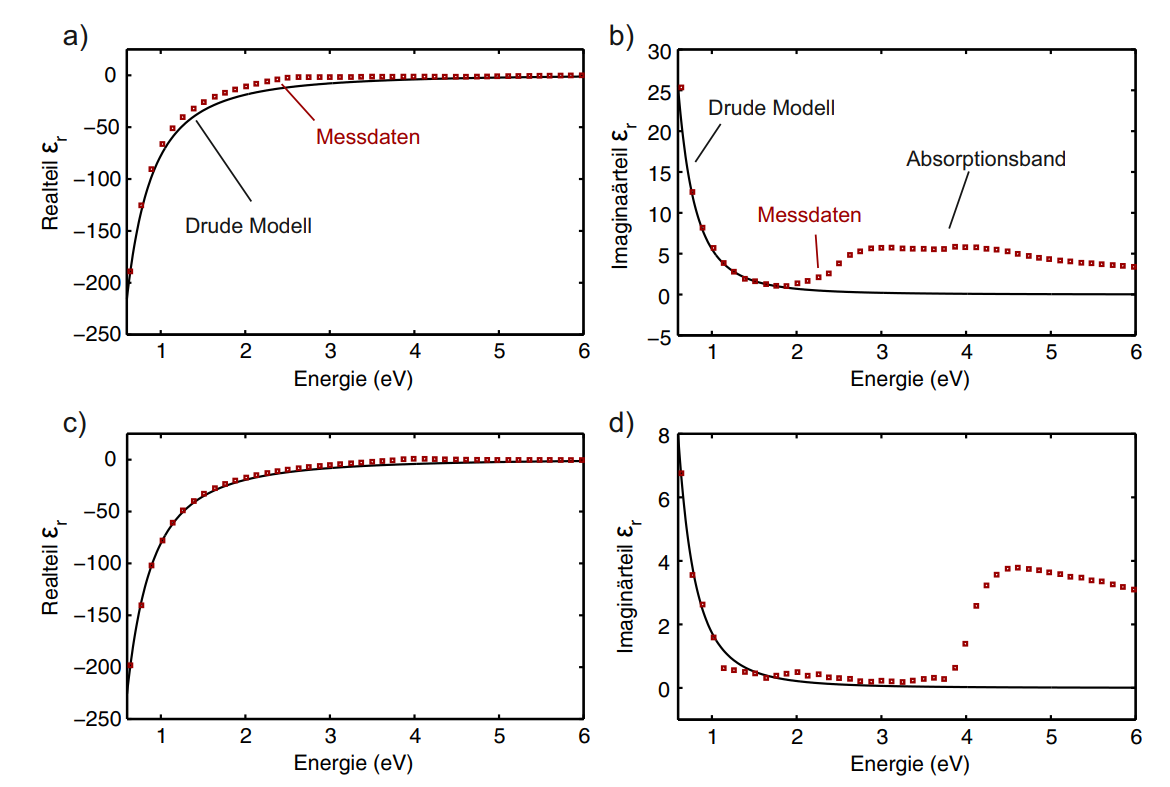
\includegraphics[width = \textwidth]{Bilder/Theory/DielectrifFuncAuS.png}
    \caption{Material-specific dielectric function $\epsilon_r$ for gold and silver. The upper graphs depict the real (a) and imaginary part (b) of gold as a function of photon energy. The red squares represent measured data by Johnson and Christy, while the black curves represent the model based on Drude's theory. Similarly, the lower graphs (c, d) display the dielectric function of silver, also measured by Johnson and Christy. Deviations from the measured values can be observed at certain energies for both metals. These deviations are caused by electron transitions (absorption bands) that are not accounted for in the model. From \cite{LehrstuhlExperimentalphysikIII.2023}}
    \label{fig:DielFuncAuS}
\end{figure}